\section{Experiments and Results}
\label{sec:experiments}


% \begin{table*}[t]
% \small
    \centering
\resizebox{1\textwidth}{!}{%
\begin{tabular}{lllllllll}
\toprule
Models &       LAMA & Group-Score &    Succ-Pat &  Succ-Objs &  Know-Const &   Unk-Const &  Const-Objs & Consistency \\

\midrule
majority-baseline &  24.2+-20.7 &  24.2+-20.7 &  100.0+-0.0 &  24.9+-20.7 &  100.0+-0.0 &  100.0+-0.0 &  100.0+-0.0 &  100.0+-0.0 \\ \midrule
bert-base         &  44.1+-25.6 &  25.0+-25.5 &  100.0+-0.0 &  60.6+-23.5 &  61.4+-23.2 &  45.2+-20.6 &  32.5+-28.5 &  57.3+-22.3 \\
bert-large        &  45.6+-27.0 &  27.5+-27.6 &   99.7+-1.8 &  63.0+-25.2 &  62.4+-22.4 &  46.4+-18.5 &  34.2+-30.0 &  59.1+-21.5 \\
bert-large-wwm    &  45.4+-26.4 &  27.2+-27.6 &  100.0+-0.0 &  61.6+-23.2 &  62.6+-23.6 &  46.5+-18.7 &  33.8+-29.8 &  58.6+-22.7 \\ \midrule
roberta-base      &  36.7+-24.6 &  16.0+-19.8 &  100.0+-0.0 &  54.2+-24.5 &  53.3+-20.2 &  41.2+-15.3 &  21.7+-23.1 &  50.1+-18.4 \\
roberta-large     &  40.8+-26.1 &  21.3+-23.7 &  100.0+-0.0 &  58.5+-24.1 &  58.2+-21.1 &  44.4+-16.0 &  27.4+-25.6 &  54.8+-19.6 \\ \midrule
albert-base       &  29.9+-24.2 &  17.0+-22.2 &   99.7+-1.8 &  45.3+-25.7 &  56.1+-21.5 &  43.1+-18.0 &  25.1+-25.4 &  51.2+-19.8 \\
albert-xxlarge    &  39.5+-26.1 &  21.9+-25.7 &   99.7+-1.8 &  56.3+-25.8 &  56.7+-22.7 &  38.8+-14.7 &  26.8+-26.8 &  51.5+-21.1 \\
\bottomrule
\end{tabular}


}
    \caption{Consistency and knowledge results for the different models.}
    \label{tab:consistency_main}
\end{table*}

\begin{table}[t]
% \small
    \centering
\resizebox{1\columnwidth}{!}{%
\begin{tabular}{lrrrr}
\toprule
Model &    Succ-Pat &   Succ-Objs &  Unk-Const &   Know-Const \\

\midrule
majority       &   97.3+-7.3 &  23.2+-21.0 &  100.0+-0.0 &  100.0+-0.0 \\
\midrule
BERT-base      &  \textbf{100.0}+-0.0 &  63.0+-19.9 &  46.5+-21.7 &  63.8+-24.5 \\
BERT-large     &  \textbf{100.0}+-0.0 &  \textbf{65.7}+-22.1 &  48.1+-20.2 &  65.2+-23.8 \\
BERT-large-wwm &  \textbf{100.0}+-0.0 &  64.9+-20.3 &  \textbf{49.5}+-20.1 &  \textbf{65.3}+-25.1 \\
\midrule
RoBERTa-base   &  \textbf{100.0}+-0.0 &  56.2+-22.7 &  43.9+-15.8 &  56.3+-19.0 \\
RoBERTa-large  &  \textbf{100.0}+-0.0 &  60.1+-22.3 &  46.8+-18.0 &  60.5+-21.1 \\
\midrule
ALBERT-base    &  \textbf{100.0}+-0.0 &  45.8+-23.7 &  41.4+-17.3 &  56.3+-22.0 \\
ALBERT-xxlarge &  \textbf{100.0}+-0.0 &  58.8+-23.8 &  40.5+-16.4 &  57.5+-23.8 \\
\bottomrule
\end{tabular}


}
    \caption{Extractability Measures, in the different models we inspect.}
    \label{tab:extractability_results}
\end{table}




\subsection{Knowledge Extraction Through Different Patterns}


% \subsection{Consistency and Knowledge}

% \yg{wdym by ``to asses the knowledge and ability of the different patterns to extract knowledge''? in particular, what is the first `knowledge'?}
% To better understand the results, and assess the knowledge and ability of the different patterns to extract the correct knowledge of \resource{}, we report additional metrics that help understanding the results. \sr{need a better motivation. e.g. ``In this section, we provide a finer-grained analysis, measuring consistency scores in various settings". But honestly this looks a bit like a checklist of different, unrelated experiments, and may be better pushed into an appendix.}

We begin by assessing the variability of our patterns as
well as the degree to which they extract the correct
entities. These results are summarized in Table
\ref{tab:extractability_results}.

First, we report \emph{Succ-Patt}, the percentage of
patterns that successfully predicted the right object at
least once. A high score  suggests that the patterns are
decent and models use  them to extract the correct
answer. We see that all PLMs achieve an almost perfect score (between 99.7\% - 100\%).
Next, we report
\emph{Succ-Objs},
the percentage of entities that were predicted correctly by at least one of the patterns.
Succ-Objs quantifies the degree to which the knowledge is stored by the models.
We see that some tuples are not predicted correctly by any of our patterns: the scores vary between 43.8\% for albert-base and 62.2 for BERT-large.
Since the average number of patterns is 8.63, i.e., there
are multiple ways to extract the knowledge, we interpret
these results as evidence that the models do not store a large part of the
\resource{} knowledge.
% \nk{This seems to suggest that it is the fault of the pattern that knowledge is not extracted from the model but an unsuccessful prediction across all models of the same tuple rather says that this knowledge is not stored} 
% The average number of factual knowledge that are correctly extracted varies between 45.3\% to 63.0\%, depending on the model. Notably, the BERT based models are consistently better than the rest in extracting the knowledge. 


% \yg{give this part a paragraph title?}
Finally, we measure \emph{Unk-Const}, consistency  for the subset of tuples
for which no pattern predicted the correct answer correctly;
and \emph{Know-Const},
consistency for the subset of tuples for which
at least one of the patterns for a specific
relation predicted the correct answer.
% A higher score on the first metric would suggest that storing the correct answer is related to the consistency of the model and performing consistent predictions across paraphrases.
Overall, the results indicate that when the factual knowledge is successfully extracted, the model is also more consistent.
For instance, for BERT-large, Know-Const  is 62.7\% and Unk-Const is 47.8\%. 
\nk{I would emphasize this even more and say that our graph is able to distinguish pattern dependent guessing and the other is knowledge stored in the model}
% point on a connection between acquiring the correct knowledge, and the ability to extract it robustly. 
% We refer to these metrics as \textsc{Know} and \textsc{Unk}, respectively, that stands for Knowledgeable and Unknowledgeable consistency.
% The additional consistent measurement we report is Const-Objs, which measures the number of tuples that are predicted consistently across all patterns for a particular relation.
% \ye{not sure if this one is important / alternatively maybe use this one instead of the main consistency score?}


\subsection{Consistency \& Knowledge}
\begin{table}[t]
% \small
    \centering
\resizebox{1\columnwidth}{!}{%
\begin{tabular}{lrrr}
\toprule
Model &        Accuracy & Consistency & Consistent-Acc \\
\midrule
majority       &  23.1+-21.0 &  100.0+-0.0 &  23.1+-21.0 \\
\midrule
BERT-base      &  45.8+-25.6 &  58.5+-24.2 &  27.0+-23.8 \\
BERT-large     &  48.1+-26.1 &  \textbf{61.1}+-23.0 &  \textbf{29.5}+-26.6 \\
BERT-large-wwm &  \textbf{48.7}+-25.0 &  60.9+-24.2 &  29.3+-26.9 \\
\midrule
RoBERTa-base   &  39.0+-22.8 &  52.1+-17.8 &  16.4+-16.4 \\
RoBERTa-large  &  43.2+-24.7 &  56.3+-20.4 &  22.5+-21.1 \\
\midrule
ALBERT-base    &  29.8+-22.8 &  49.8+-20.1 &  16.7+-20.3 \\
ALBERT-xxlarge &  41.7+-24.9 &  52.1+-22.4 &  23.8+-24.8 \\
\bottomrule
\end{tabular}



}
    \caption{Knowledge and Consistency Results. Best model for each metric is highlighted in bold.}
    \label{tab:consistency_results_small}
\end{table}


 In this section, we report
the overall knowledge measure that was used in \citet{lama},
our consistency results, as well as a new measure that
combines both knowledge and consistency measures.  The
results are summarized in Table
\ref{tab:consistency_results_small}.

We begin with the LAMA results, that is, the acc@1 of a
model in predicting the object, using the original patterns
from \citet{lama}. acc@1 is defined as accuracy of the
top-ranked object within the candidate set of each
relation. Our numbers differ from \citet{lama} as we use a
candidate set (\S\ref{sec:probe}) and only consider KB
triples whose object is a single token
(\S\ref{setupdata}). The results range between 28.4\%
(albert-base) and 45.0\% (bert-large whole-word-masking).

Next, we report the consistency measure (\S\ref{sec:eval}).
BERT-based models achieve the highest scores. There is a consistent improvement from the {base} to {large} versions of each model.
% , although it is not always significantly \am{is there a significance test?} higher (e.g. 57.3\% to 59.1\% in BERT, and 50.1\% to 54.8\% in RoBERTa).
In contrast to much previous work that observed quantitative and qualitative improvements of RoBERTa-based models over BERT, in terms of consistency, BERT is more consistent than RoBERTa and ALBERT.
Still, the overall results are remarkably low (59.6\% for
the best model), %\yg{meaning that out of XXX, YYY are
%ZZZ}),
even more remarkably so because the restricted candidate set
makes the task easier.
We note that the results are highly variant between models
(the best performance of any of the models on
`capital of' is 94\% whereas it is 44\% for `owned by')
and relations (models' performance on `original language of film or TV show'  varies between 52\% and 90\%).
% We report the full consistency results for each relation in the Appendix.

Finally, we report
\emph{Group-Score}: it evaluates an object as correct only
if \emph{all} patterns predict the object
correctly. Group-Score is much stricter and it combines  the
requirements
of consistency and factual correctness.
The results are much lower than  LAMA acc@1, as expected,
but follow the same trend: albert-base perform worse (15.8\%) and bert-large  best  (26.8\%).





% For brevity, we report the results solely on BERT-large, which achieved the highest results. The results can be viewed in Table \ref{tab:bert-results}.

A striking result of the model comparison is
the clear superiority of
BERT, both in knowledge accuracy and knowledge
consistency. This result, which we hypothesise to be due to
the training data, may have a broader impact on models to
come: Training bigger models with more data is not always
beneficial. Since Wikipedia is likely the largest unified source
of factual knowledge that exists in unstructured data,
giving prominence to Wikipedia in pretraining a model makes it more
likely that the model will incorporate the factual knowledge
well. 
This may indicate that  the consistency of models such as GPT-3 \cite{gpt3}
or other future models -- i.e., models that
have a much larger size and
are trained on very large corpora of
which Wikipedia is just a small part -- may suffer.

% \am{this is unsubstantiated, you can add "we hypothesize" to make this claim}% and retain more factual knowledge.




%%%%%%%%%%%%%%%%%%%%%%%%%%%%%%%%5



% \subsection{Consistency}

% The results for the different models are summarized in Table \ref{tab:consistency_main}.
% % First, we report the average consistency results for all graphs, as describe in Section \ref{sec:eval}.
% The last column (``Consistency'') shows the average results across all relations \yg{consider oredering the table columns in the order of their discussion}\am{I actually like it in the end, its easier to find in a glance}



\begin{table}[t]
% \small
    \centering
\resizebox{1\columnwidth}{!}{%
\begin{tabular}{lrrr}
\toprule
Model&        Acc & Consistency & Consistent-Acc \\

\midrule
majority               &  23.1+-21.0 &  100.0+-0.0 &  23.1+-21.0 \\
\midrule
RoBERTa-med-small-1M &   11.2+-9.4 &  37.1+-11.0 &    2.8+-4.0 \\
\midrule
RoBERTa-base-10M     &  17.3+-15.8 &  29.8+-12.7 &    3.2+-5.1 \\
RoBERTa-base-100M    &  22.1+-17.1 &  31.5+-13.0 &    3.7+-5.3 \\
RoBERTa-base-1B      &  \textbf{38.0}+-23.4 &  \textbf{50.6}+-19.8 &  \textbf{18.0}+-16.0 \\
\bottomrule
\end{tabular}
}
    \caption{Knowledge and consistency results for the different RoBERTas, trained on increasing amounts of data. Best model for each metric is highlighted in bold.}
    \label{tab:robertas}
\end{table}

% \enote{hs}{below: i would prefer ``(training) corpus size''
%   over ``number of tokens'' if that's what you mean}

\paragraph{Effect of Pretraining Corpus Size}
Next, we study the question of whether the number of tokens used during pretraining contributes to consistency.
We use the pretrained RoBERTa model provided by \citet{robertas} and repeat the experiments on four additional models.
These models are RoBERTa-based models that were trained on a sample of Wikipedia and the book corpus, with varying training size and parameters. We use one of the three published models for each configuration and report the average accuracy over the relations for each model in Table \ref{tab:robertas}.
Overall, the consistency and the knowledge scores (LAMA and
Group-Score) improve
with more training data.
However, there is an interesting outlier to this trend.
First, the model that was trained on one million tokens is
more consistent than the models trained on ten and
one-hundred million tokens. A potentially crucial difference
is that this model
has many fewer parameters than the rest (to avoid overfitting). It is nonetheless interesting that a model that is trained on significantly less data can achieve better consistency. On the other hand, the knowledge scores are lower, arguably due to the model being exposed to less factual knowledge during pretraining.

% Finally, the original RoBERTa that was trained on ten billion parameters, achieves the same consistency performance as the one trained on one billion tokens, suggesting a limit to the benefit of training examples in pretraining. \nk{not sure about this as the table is not there yet, but shouldn't it be: Finally, the original RoBERTa that was trained on ten billion tokens, achieves the same consistency performance as the one trained on one billion tokens, suggesting on a limit to the benefit of large training corpora. }



% \begin{table*}[t]
% \small
    \centering
\resizebox{1\textwidth}{!}{%
\begin{tabular}{lrrrrrrr}
\toprule
{} &  bert-base &  bert-large &  bert-large-wwm &  roberta-base &  roberta-large &  albert-base &  albert-xxlarge \\
\midrule
syn   &             0.50 &              0.53 &                                 0.53 &          0.44 &           0.48 &            0.44 &               0.45 \\
lex   &             0.56 &              0.59 &                                 0.58 &          0.51 &           0.54 &            0.52 &               0.49 \\
both  &             0.72 &              0.72 &                                 0.72 &          0.67 &           0.68 &            0.70 &               0.63 \\ \midrule
total &             0.52 &              0.54 &                                 0.54 &          0.45 &           0.50 &            0.46 &               0.46 \\
\bottomrule
\end{tabular}


}
    \caption{Consistent results aggregated on the different relations, by the different splits.}
    \label{tab:entailment-splits}
\end{table*}

% \begin{table*}[t]
% \small
    \centering
\resizebox{1\textwidth}{!}{%
\begin{tabular}{llrrrrrrr}
\toprule
     type & index &  bert-base-cased &  bert-large-cased &  bert-large-cased-wwm &  roberta-base &  roberta-large &  albert-base &  albert-xxlarge \\
\midrule
\multirow{3}{*}{consistency} & 1-1 &             0.76 &              0.82 &                                 0.84 &          0.58 &           0.73 &            0.66 &               0.80 \\
     & N-1 &             0.55 &              0.56 &                                 0.57 &          0.48 &           0.51 &            0.46 &               0.48 \\
     & N-M &             0.43 &              0.47 &                                 0.46 &          0.39 &           0.44 &            0.44 &               0.40 \\
\cline{1-9}
\multirow{3}{*}{syntactic} & 1-1 &             0.75 &              0.81 &                                 0.83 &          0.57 &           0.72 &            0.66 &               0.79 \\
     & N-1 &             0.53 &              0.55 &                                 0.56 &          0.46 &           0.49 &            0.44 &               0.47 \\
     & N-M &             0.41 &              0.45 &                                 0.44 &          0.38 &           0.43 &            0.42 &               0.40 \\
\cline{1-9}
\multirow{3}{*}{lexical} & 1-1 &             0.85 &              0.88 &                                 0.89 &          0.67 &           0.80 &            0.75 &               0.86 \\
     & N-1 &             0.59 &              0.60 &                                 0.62 &          0.55 &           0.57 &            0.51 &               0.51 \\
     & N-M &             0.45 &              0.53 &                                 0.48 &          0.40 &           0.44 &            0.52 &               0.39 \\
\cline{1-9}
\multirow{3}{*}{both} & 1-1 &             0.59 &              0.76 &                                 0.83 &          0.16 &           0.49 &            0.46 &               0.73 \\
     & N-1 &             0.75 &              0.76 &                                 0.74 &          0.69 &           0.72 &            0.72 &               0.69 \\
     & N-M &             0.68 &              0.66 &                                 0.68 &          0.64 &           0.64 &            0.68 &               0.54 \\
\bottomrule
\end{tabular}

}
    \caption{Consistent results aggregated on the different relations, by the different splits.}
    \label{tab:entailment-splits}
\end{table*}


% \begin{figure*}[t!]
% \centering

% 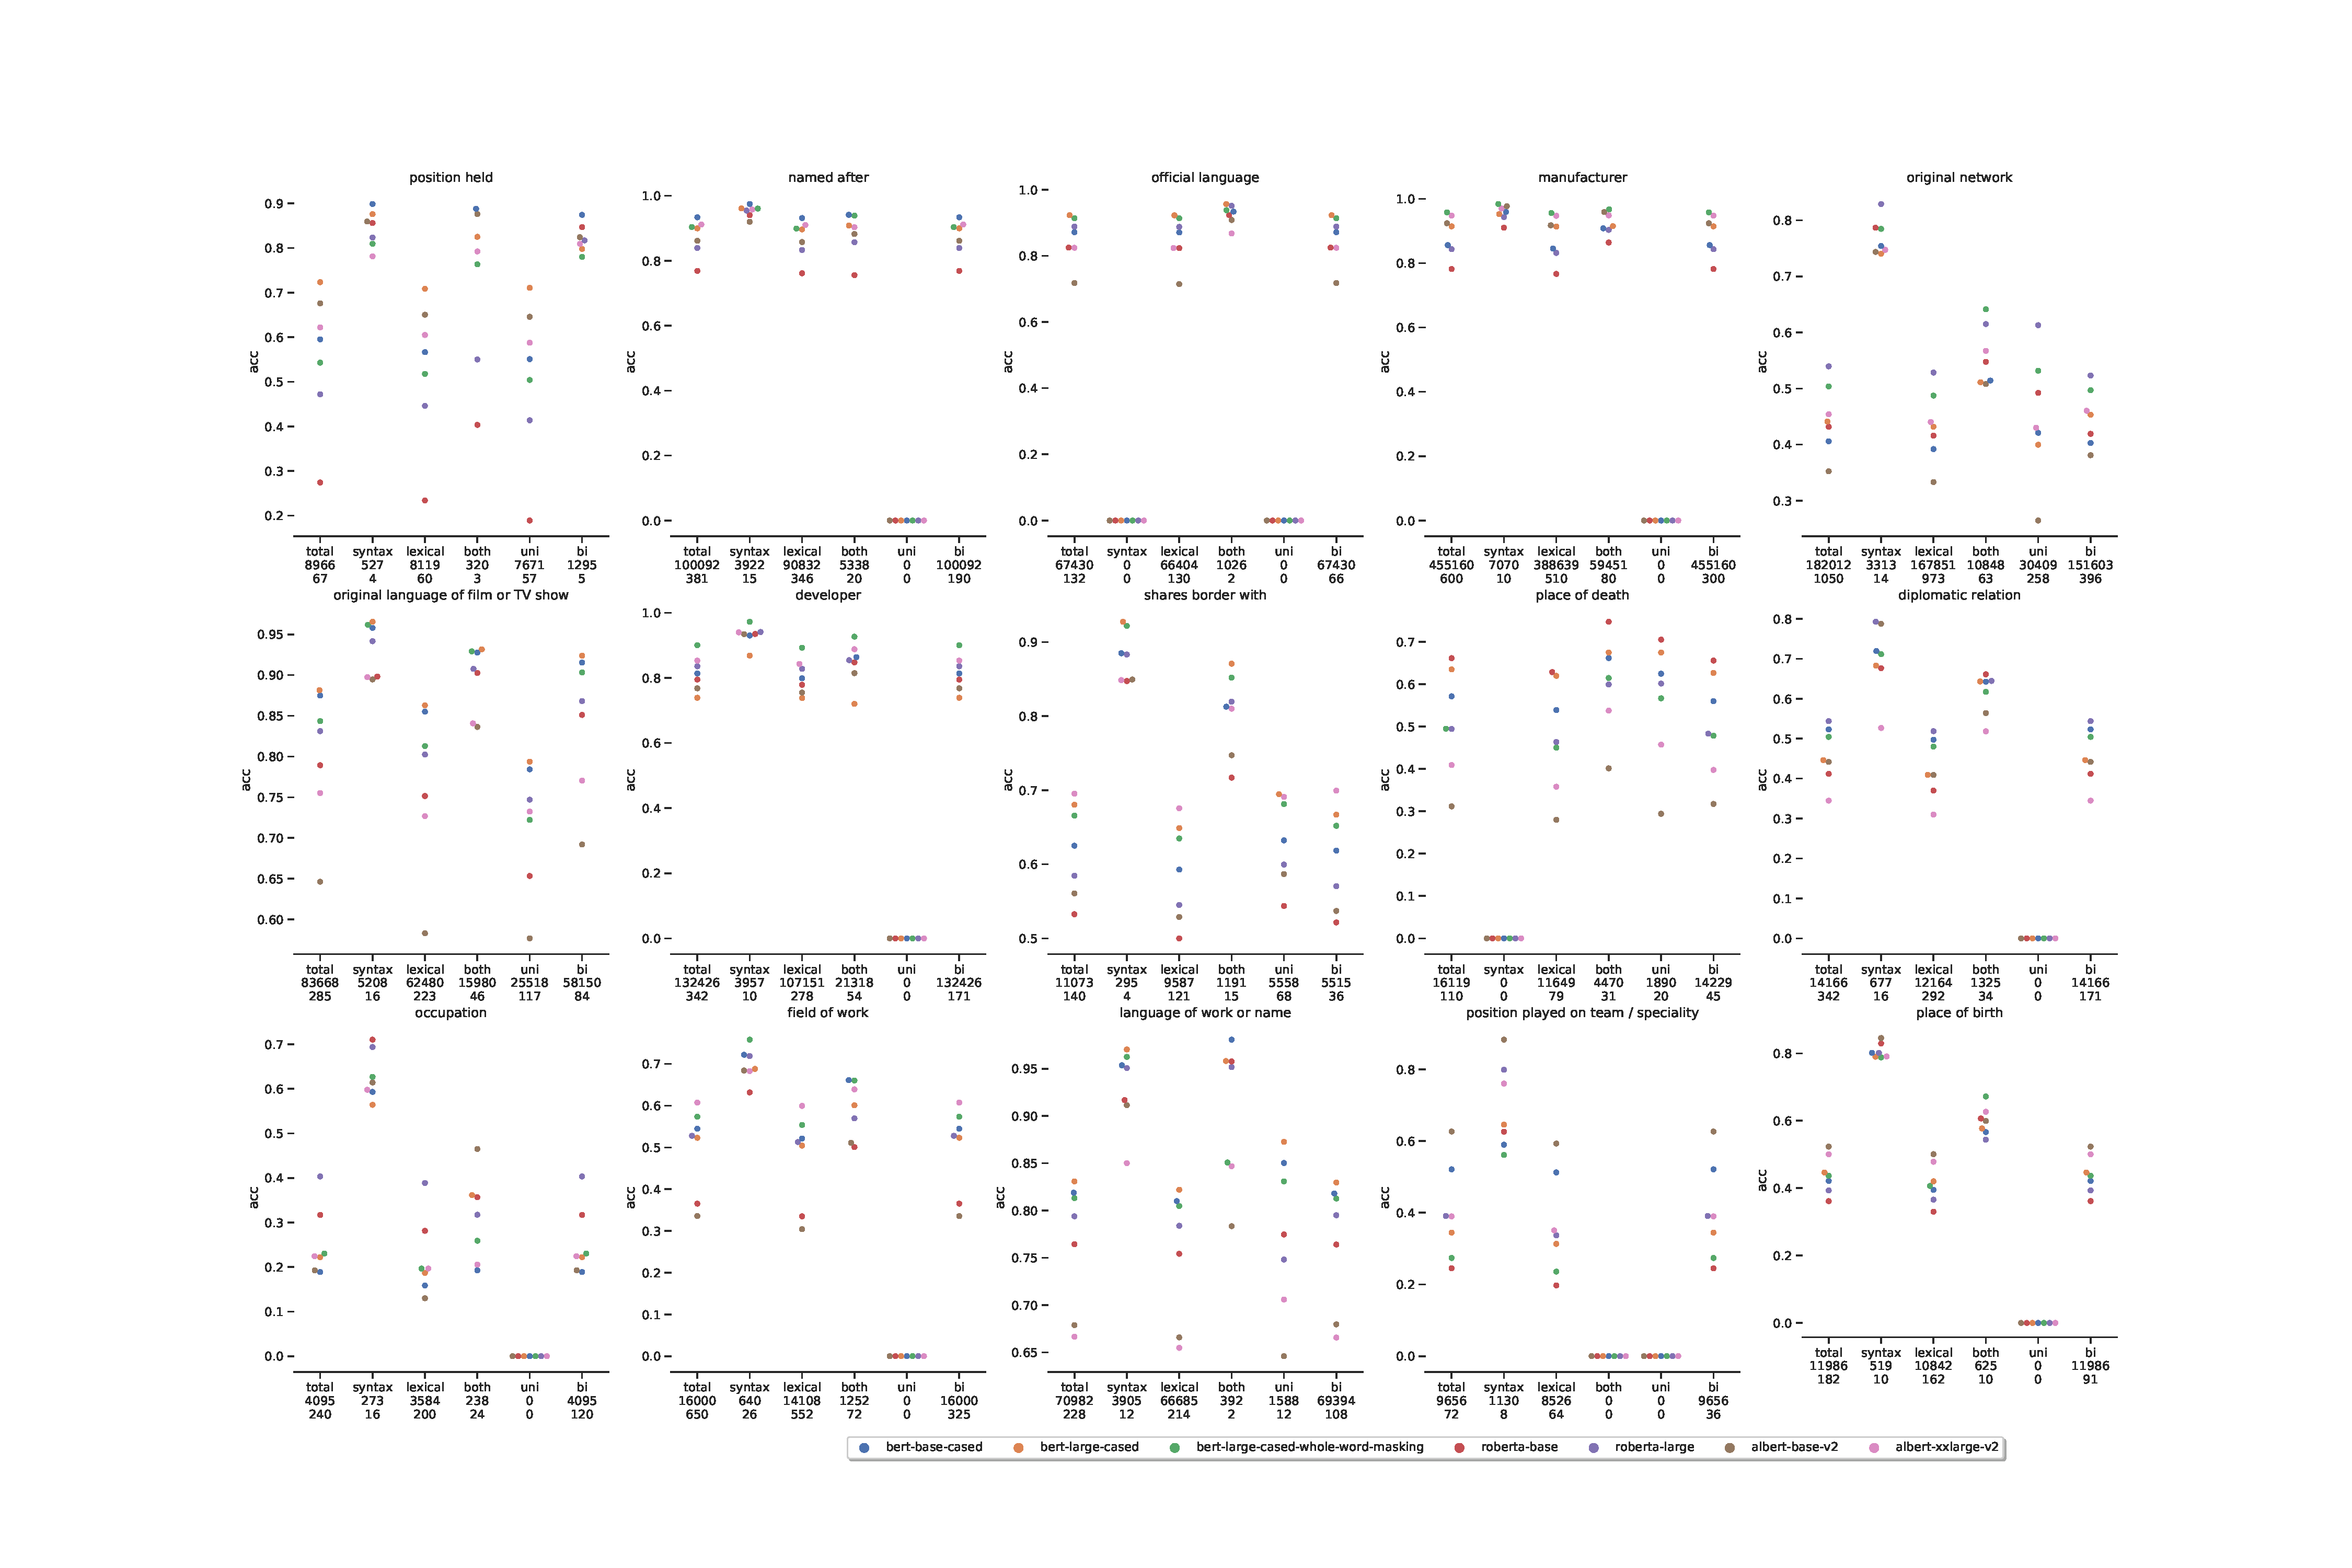
\includegraphics[width=1.\textwidth]{figures/results}

% \caption{Results summary, by relation, by split.}
% \label{fig:resuls}
% % \vspace{-6mm}
% \end{figure*}

% \begin{table*}[t]
% \small
    \centering
\resizebox{1\textwidth}{!}{%
\begin{tabular}{lrrrrrrrr}
\toprule
                              pattern &  know &  unk &  top@1 &  group-score &  const-subjs &  succ-patt &  succ-subjs &  consistency \\
\midrule
                             religion &                      0.35 &                        0.22 &      0.12 &            0.09 &                 0.09 &                  1.0 &                 0.88 &         0.34 \\
                       place of death &                      0.43 &                        0.32 &      0.42 &            0.04 &                 0.05 &                  1.0 &                 0.54 &         0.38 \\
                              capital &                      0.91 &                        0.40 &      0.70 &            0.57 &                 0.61 &                  1.0 &                 0.75 &         0.78 \\
                           instrument &                      0.48 &                        0.62 &      0.50 &            0.03 &                 0.05 &                  1.0 &                 0.85 &         0.50 \\
                             employer &                      0.38 &                        0.38 &      0.10 &            0.03 &                 0.11 &                  1.0 &                 0.27 &         0.38 \\
                headquarters location &                      0.65 &                        0.35 &      0.36 &            0.21 &                 0.25 &                  1.0 &                 0.53 &         0.51 \\
                        position held &                      0.49 &                        0.46 &      0.29 &            0.08 &                 0.11 &                  1.0 &                 0.65 &         0.48 \\
                            continent &                      0.92 &                        0.74 &      0.90 &            0.83 &                 0.85 &                  1.0 &                 0.97 &         0.91 \\
                            member of &                      0.92 &                        0.27 &      0.84 &            0.72 &                 0.74 &                  1.0 &                 0.89 &         0.85 \\
                              country &                      0.89 &                        0.74 &      0.60 &            0.54 &                 0.77 &                  1.0 &                 0.65 &         0.84 \\
                          subclass of &                      0.83 &                        0.53 &      0.61 &            0.56 &                 0.63 &                  1.0 &                 0.78 &         0.76 \\
                          instance of &                      0.51 &                        0.19 &      0.53 &            0.05 &                 0.05 &                  1.0 &                 0.86 &         0.47 \\
                              part of &                      0.62 &                        0.53 &      0.47 &            0.31 &                 0.57 &                  1.0 &                 0.51 &         0.57 \\
                             owned by &                      0.55 &                        0.23 &      0.51 &            0.21 &                 0.22 &                  1.0 &                 0.65 &         0.44 \\
                         record label &                      0.26 &                        0.28 &      0.06 &            0.00 &                 0.00 &                  1.0 &                 0.79 &         0.26 \\
                        field of work &                      0.28 &                        0.21 &      0.15 &            0.01 &                 0.01 &                  1.0 &                 0.39 &         0.23 \\
                        work location &                      0.74 &                        0.68 &      0.42 &            0.28 &                 0.42 &                  1.0 &                 0.59 &         0.72 \\
             language of work or name &                      0.70 &                        0.60 &      0.72 &            0.21 &                 0.23 &                  1.0 &                 0.85 &         0.69 \\
          twinned administrative body &                      0.57 &                        0.70 &      0.04 &            0.02 &                 0.37 &                  1.0 &                 0.07 &         0.69 \\
                         manufacturer &                      0.88 &                        0.33 &      0.90 &            0.62 &                 0.62 &                  1.0 &                 0.96 &         0.86 \\
                location of formation &                      0.59 &                        0.50 &      0.11 &            0.03 &                 0.13 &                  1.0 &                 0.18 &         0.52 \\
                                genre &                      0.52 &                        0.41 &      0.61 &            0.03 &                 0.03 &                  1.0 &                 0.79 &         0.49 \\
                    official language &                      0.87 &                        0.70 &      0.64 &            0.49 &                 0.64 &                  1.0 &                 0.81 &         0.84 \\
 position played on team / speciality &                      0.30 &                        0.32 &      0.06 &            0.00 &                 0.00 &                  1.0 &                 0.45 &         0.31 \\
                            developer &                      0.63 &                        0.28 &      0.71 &            0.22 &                 0.22 &                  1.0 &                 0.91 &         0.60 \\
                             location &                      0.56 &                        0.34 &      0.49 &            0.01 &                 0.01 &                  1.0 &                 0.70 &         0.49 \\
                          named after &                      0.78 &                        0.47 &      0.60 &            0.38 &                 0.41 &                  1.0 &                 0.80 &         0.71 \\
                    country of origin &                      0.67 &                        0.54 &      0.40 &            0.20 &                 0.25 &                  1.0 &                 0.63 &         0.62 \\
                     original network &                      0.29 &                        0.25 &      0.33 &            0.00 &                 0.00 &                  1.0 &                 0.82 &         0.28 \\
                       place of birth &                      0.46 &                        0.38 &      0.26 &            0.00 &                 0.01 &                  1.0 &                 0.32 &         0.41 \\
              applies to jurisdiction &                      0.94 &                        0.69 &      0.76 &            0.74 &                 0.82 &                  1.0 &                 0.83 &         0.90 \\
                           occupation &                      0.34 &                        0.35 &      0.01 &            0.00 &                 0.00 &                  1.0 &                 0.14 &         0.35 \\
                           capital of &                      0.95 &                        0.51 &      0.89 &            0.80 &                 0.82 &                  1.0 &                 0.92 &         0.92 \\
 original language of film or TV show &                      0.89 &                        0.90 &      0.58 &            0.50 &                 0.79 &                  1.0 &                 0.64 &         0.90 \\
               country of citizenship &                      0.74 &                        0.65 &      0.36 &            0.27 &                 0.32 &                  1.0 &                 0.68 &         0.71 \\
                   shares border with &                      0.54 &                        0.54 &      0.26 &            0.06 &                 0.14 &                  1.0 &                 0.54 &         0.54 \\
\bottomrule
\end{tabular}
}
    \caption{Additional results for the BERT-large model. }
    \label{tab:bert-results}
\end{table*}



\enote{hs}{below: many people might think that a difference
  in tense is a difference in syntax. Tense is part of
  syntax?
}

\subsection{Do PLMs Generalize Over Syntax?} 

\begin{table}[t]
% \small
    \centering
\resizebox{0.8\columnwidth}{!}{%
\begin{tabular}{lll}
\toprule
Model & Diff-Syntax & No-Change \\
\midrule
majority       &            100.0+-0.0 &            100.0+-0.0 \\
\midrule
BERT-base      &            67.9+-30.3 &            76.3+-22.6 \\
BERT-large     &            67.5+-30.2 &            78.7+-14.7 \\
BERT-large-wwm &            63.0+-31.7 &             \textbf{81.1}+-9.7 \\
\midrule
RoBERTa-base   &            66.9+-10.1 &             80.7+-5.2 \\
RoBERTa-large  &            \textbf{69.7}+-19.2 &             80.3+-6.8 \\
\midrule
ALBERT-base    &            62.3+-22.8 &            72.6+-11.5 \\
ALBERT-xxlarge &            51.7+-26.0 &            67.3+-17.1 \\
\bottomrule
\end{tabular}

}
    \caption{Consistency and standard deviation when only syntax differs
      (\textit{Diff-Syntax}) and when syntax and lexical choice are identical (\textit{No-Change}). Best model for each metric is highlighted in bold.}
    \label{tab:syntax_results}
\end{table}


Many papers have found models (especially PLMs) to naturally
encode syntax
\cite{linzen2016assessing,marvin-linzen-2018-targeted,yoav-syntax,hewitt2019structural}.
%How does this reflect in their ability to abstract
%knowledge and produce it while controlling for syntactic
%variations?
Does this mean that PLMs have successfully abstracted
knowledge and can comprehend and produce it regardless of
syntactic variation?
We consider two scenarios. (1) two patterns differ only in
syntax. (2) Both  syntax and  lexical choice are the same.
Here we define identical syntax as identical dependency
paths between subject and object.
We parse all patterns from \resource{} using a dependency parser \cite{spacy}\footnote{\url{https://spacy.io/}} and retain the path between  subject and object.

Success on (1) indicates
that the model's knowledge processing is robust to syntactic
variation.
Success on (2) indicates
that the model's knowledge processing is robust to
variation in word order and tense.

%the ability of the model to abstract the knowledge, and extract it using different syntactic patterns. Success on (2) indicates the abstraction over word order and tense. This way, we can test for consistency in models, while controlling for syntactic variation.\footnote{We consider two patterns to have the same syntax if the path between the entities are equal} 
% \sr{needs a footnote on our \emph{proxy} for syntactic change.}
% staying invariant to alternations while the syntax is the only component that differs, and when 
% Then, for every pattern pair, we split into two groups: (1) patterns where the only difference is the syntactic path, but the lexical items are equal, and (2) patterns where both the syntactic path and the lexical items are identical. \nk{This sentence seems repetitive}
% we filter out all cases where the syntactic path is different. 


Table \ref{tab:syntax_results}
reports results.
While the results are not comparable to the main results on
the entire dataset as the pattern subsets are different, overall
the results are low: 61.5\% for BERT-large when only 
syntax differs, and 78.7\% when syntax is
identical.  This demonstrates that while PLMs have impressive syntactic
abilities, 
they struggle to extract factual knowledge in the face of
tense, word-order and syntactic variation.

% These results are surprising, since the ability to abstract over syntax is perhaps the easier abstraction, and was expected to perform better, given other results on PLMs syntactic abilities. \sr{not sure if we can say it's easier/harder.}

\citet{mccoy2019right}  show that supervised models trained on an NLI
dataset \cite{dagan-rte,snli} such as MNLI \cite{mnli} use
superficial syntactic heuristics rather than more
generalizable properties of the data.
Our results show that pretrained PLMs have  problems along
the same lines:
they are not robust to surface variation.

%These results reminiscent of the findings of
%However, we demonstrate that even PLMs are susceptible to these errors. 
